\chapter{Introduction}

\section{Caching Problem}

Storing data in a faster storage medium to serve future requests faster for that data is a 
very common technique in computer science called caching. We will consider the problem 
of caching of pages of fixed size in a buffer pool of fixed size.

We call cache hit when the requested page is already in the cache, and cache fault or miss
when the requested page is not in the cache. Generally, the goal is to maximize the number
of cache hits.

When a page is accessed, and the buffer is full, we need to decide which page to evict
from the cache to make space for the new page. This is called the cache eviction policy,
and it is a crucial part of the caching problem.

The optimal cache eviction policy is to evict the page that will be requested the farthest
in the future \cite{lecture-notes-1} \cite{lecture-notes-2} \cite{article-for-belady-ref-1}.
But this is impractical in most cases, since it is generally impossible to predict how
far in the future a page will be requested.

Several cache eviction policies have been developed, which incorporate information
about recency and/or frequency of page requests to make eviction decisions, we will
discuss some of them in detail in the following chapters.

\section{Buffer Sharing in Multi-Tenant Caches}

In a multi-tenant environment, multiple tenants share the same buffer pool. Proper 
allocation of the buffer pool among tenants is crucial for the performance of each
tenant workload \cite{buffer-sharing-1}.

In this thesis, we will consider the problem of buffer sharing in multi-tenant caches,
where each tenant has completely different workloads, data of one tenant is completely
independent of the data of another tenant.

We mainly consider small number of tenants, since it is common in possible applications, 
experiments based on real data have 4 or 5 tenants, experiments on random data have up 
to 10 tenants, however, the proposed algorithms also work for larger number of tenants.

\subsection{Global, Static and Dynamic Buffer Allocation}

Some of the main approaches to buffer allocation in multi-tenant caches are:

\begin{enumerate}
    \item Global Buffer Allocation: All tenants share the same buffer pool, and the 
    buffer allocation is fixed. This approach is very simple and easy to implement,
    but it allows unlimited sharing of the buffer, and hence, it becoomes difficult to 
    guarantee the specified performance goal for individual tenants
    \cite{article-for-2level-forecasting} (Fig \ref{fig:figA-1}).
    \item Static Buffer Allocation: Each tenant has a fixed buffer size, and the buffer
    allocation is fixed. While straightforward to manage without sharing, a critical 
    downside of static caching is that it is hard to estimate the required amount of 
    the cache space in advance \cite{article-for-2level-forecasting} (Fig \ref{fig:figB-1}).
    \item Dynamic Buffer Allocation: The size of cache space for a tenant is adjusted 
    over time by monitoring performance. For this, it is critical to have good seasonality
    recommendations of cache sizes per tenant. Inadequate predictions will lead to the waste
    of resources or the failure of the performance guarantee \cite{article-for-2level-forecasting}
    There have been various studies to address this problem, such as based on the 
    approximation to concave functions \cite{approx-concave-functions} and a 
    learning-based prediction \cite{learning-based-prediction}, but it is still a 
    challenging problem to make accurate estimations of access patterns with an 
    acceptable error bound.
\end{enumerate}

\begin{figure}[H]
    \centering
    \begin{minipage}{0.4\textwidth}
        \centering
        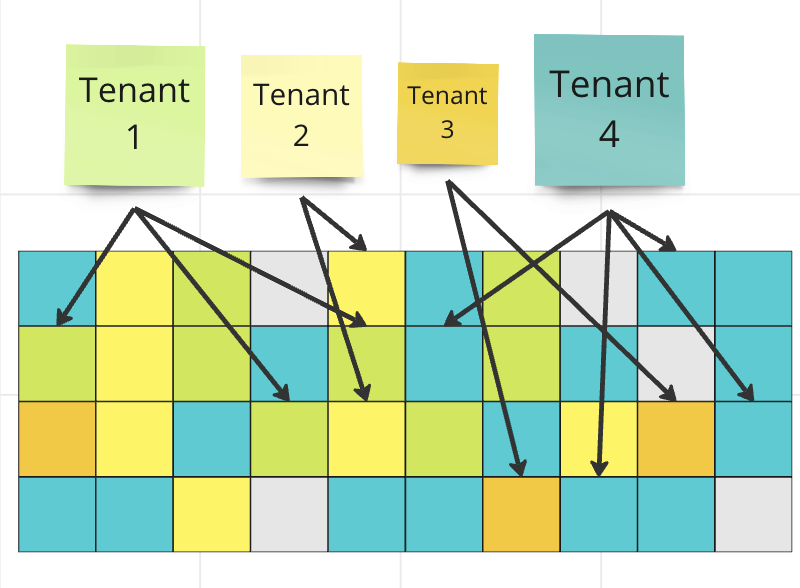
\includegraphics[width=\textwidth]{global_cache.png}
        \caption{Global Caching}
        \label{fig:figA-1}
    \end{minipage}
    \hfill
    \begin{minipage}{0.4\textwidth}
        \centering
        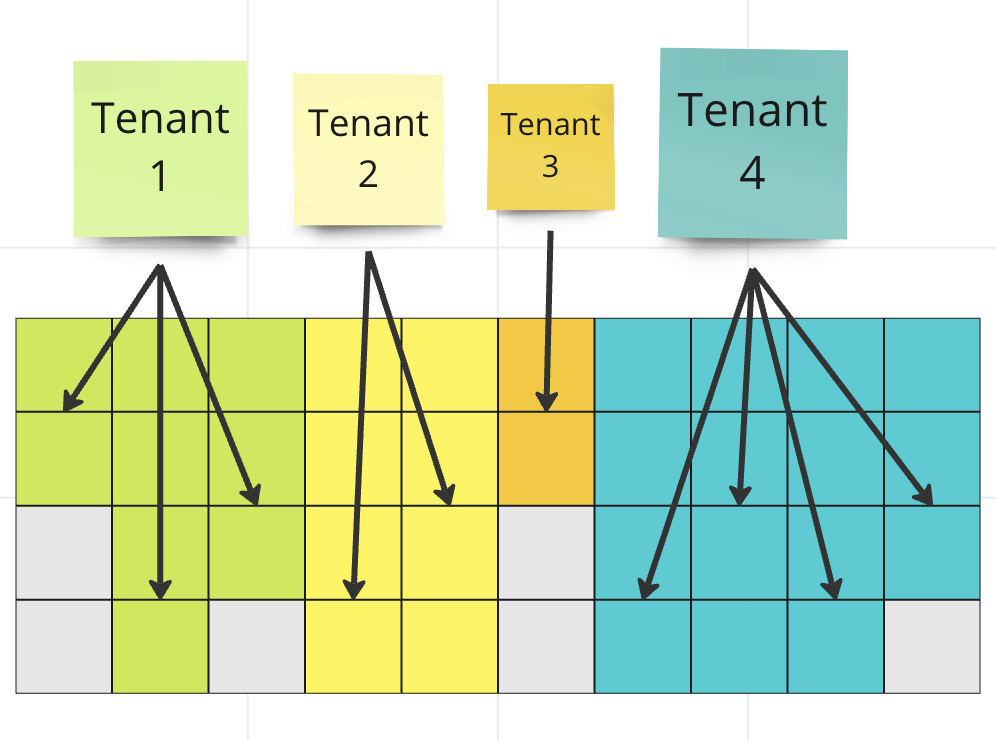
\includegraphics[width=\textwidth]{static_cache.png}
        \caption{Static Caching}
        \label{fig:figB-1}
    \end{minipage}
\end{figure}

The main case of study in this thesis is the dynamic buffer allocation, therefore our
caching policy will be adaptive to the buffer allocation of each tenant.

\subsection{Two level forecasting algorithm}

Since we are mainly interested in dynamic buffer allocation, caching problem in this
case can be seen as a two level forecasting problem. The first level is the seasonality
recommendation algorithm, which gives the buffer allocation of each tenant, and the
second level is the eviction policy, which makes eviction decisions based on the buffer
allocation.

The main focus of this thesis is on the eviction policy, for that, we will assume that
the buffer recommendations are given, and we will compare the performance of different
eviction policies.

While the recommendations are given, this does not mean that will have the cache problem
like single caches with fixed size, since the buffer allocation of each tenant is a 
recommendation that does not needs to be followed exactly, and it will also change
over time, therefore our eviction policy needs to be adaptive to the buffer allocation
of each tenant.

\subsection{Application to Multi-Tenant Relational Databases}

Relational database systems are widely used in many enterprises to store, manage and 
query data in applications in a structured way. Several commercial cloud relational
database services, such Google Cloud SQL \cite{google-cloud-sql}, Microsoft Azure SQL 
Database \cite{azure-sql}, and Oracle Cloud Database \cite{oracle-cloud} have emerged. 

In this cloud services, multi tenancy is crucial to increase consolidation and reduce
cost by sharing resources among tenants \cite{buffer-sharing-1}.

A database as a service (DaaS) provider would like to overbook the resources, i.e. 
promise more resources to tenants in aggregate than is physically available on the
machine, yet without affecting tenant performance. This is based on the observation 
that at any point in time some tenants on the machine are likely to use much fewer 
resources than they are promised. \cite{buffer-sharing-1} The main challenge is to 
allocate resources to tenants in a way that guarantees the performance of each tenant 
workload.

\section{Cost function optimization}

\lipsum[1-1] \cite{reference-3}

\section{Research Question}

\begin{table}[ht!]
    \centering
    \begin{tabular}{c c c}
        \hline
        Column 1 & Column 2 & Column 3 \\
        \hline
        Item 1   & Item 2   & Item 3   \\
    \end{tabular}
    \caption{Lorem ipsum dolor sit amet}
    \label{tab:tabA-1}
\end{table}

\lipsum[1-1] \ref{tab:tabA-1}

\begin{table}[ht!]
    \centering
    \begin{tabular}{c c c}
        \hline
        Column 1 & Column 2 & Column 3 \\
        \hline
        Item 1   & Item 2   & Item 3   \\
    \end{tabular}
    \caption{Lorem ipsum dolor sit amet}
    \label{tab:tabB-1}
\end{table}

\lipsum[1-1] \ref{tab:tabB-1}

\section{Objectives}

\lipsum[1-2]

\section{Outline}

\lipsum[1-2]